%*******************************************************************************
% Title: Ontoqa, Q&A with ontology-based natural language processing
%
% Conference: Courseworks in Artificial Intelligence
%
% Author: Antonella Botte <abotte@acm.org>
% Author: Giacomo Marciani <gmarciani@acm.org>
% Author: Debora Partigianoni <dpartigianoni@acm.org>
%
% Institution: Department of Civil Engineering and Computer Science Engineering,
%         University of Rome Tor Vergata, Italy
%
% Style: ACM Large VERSION 2017
%*******************************************************************************

\documentclass[acmlarge]{acmart}

%*******************************************************************************
% Packages
%*******************************************************************************
\usepackage[utf8]{inputenc}
\usepackage{amsmath}
\usepackage{booktabs}
\usepackage{lipsum}
\usepackage{xr}

%*******************************************************************************
% Meta
%*******************************************************************************
\acmJournal{ACMROME-CP}
\acmVolume{1}
\acmNumber{1}
\acmArticle{1}
\acmYear{2017}
\acmMonth{2}
\acmArticleSeq{11}
\acmDOI{0000001.0000001}
\acmPrice{0.00}
\received[accepted]{February 2017}

%*******************************************************************************
% Copyright
%*******************************************************************************
\setcopyright{rightsretained}

%*******************************************************************************
% Algorithm
%*******************************************************************************
\usepackage[ruled]{algorithm2e}
\renewcommand{\algorithmcfname}{ALGORITHM}
\SetAlFnt{\small}
\SetAlCapFnt{\small}
\SetAlCapNameFnt{\small}
\SetAlCapHSkip{0pt}
\IncMargin{-\parindent}

%*******************************************************************************
% Custom Commands
%*******************************************************************************

%*******************************************************************************
% Numbering
%*******************************************************************************
\numberwithin{equation}{section}

%*******************************************************************************
% References
%*******************************************************************************
\externaldocument{sec/introduction}
\externaldocument{sec/overview}
\externaldocument{sec/architecture}
\externaldocument{sec/implementation}
\externaldocument{sec/evaluation}
\externaldocument{sec/improvements}
\externaldocument{sec/conclusions}

\begin{document}
%*******************************************************************************
% Title and Authors
%*******************************************************************************
\title{Ontoqa, Q\&A with ontology-based natural language processing}
\author{Antonella Botte}
\orcid{0000-0000-0000-0000}
\affiliation{%
  \institution{University of Rome Tor Vergata}
  \streetaddress{Via del Politecnico 1}
  \city{Rome}
  \state{RM}
  \postcode{00133}
  \country{IT}}
\author{Giacomo Marciani}
\orcid{0000-0002-3675-8804}
\affiliation{%
  \institution{University of Rome Tor Vergata}
  \streetaddress{Via del Politecnico 1}
  \city{Rome}
  \state{RM}
  \postcode{00133}
  \country{IT}}
\author{Debora Partigianoni}
\orcid{0000-0000-0000-0000}
\affiliation{%
  \institution{University of Rome Tor Vergata}
  \streetaddress{Via del Politecnico 1}
  \city{Rome}
  \state{RM}
  \postcode{00133}
  \country{IT}}

%*******************************************************************************
% Front
%*******************************************************************************
\begin{abstract}
	
% MOTIVATION
Natural language processing (NLP) is a family of technologies that can disruptively reshape human-machine interaction, data-driven decision making and daily exploration of knowledge by humans.
%
One of the most representative and widely studied NLP application is question-answering (Q\&A).
%
With the fast growing diffusion of semantic web and advancement in NLP technologies, Q\&A systems will be one of the most important interface to knowledge.


% PROBLEM STATEMENT
Since it is not possible to develop a single ontology to effectively capture the whole knowledge, it is necessary to develop Q\&A systems that can easily adapt to distinct ontologies and lexicons.


% APPROACH
In this work we describe Ontoqa, a Q\&A web and standalone application which aims to achieve this ambitious goal.
%
The proposed solution leverages ontology-driven NLP through the use of the LTAG/DUDES model and a greedy parsing algorithm aiming to reduce both the syntactic and semantic search space.
%
%
% RESULTS
The experimental results show that our system can answer the benchmark questions, with good performance with respect to both response-time and memory usage. 
%
%
% CONCLUSIONS
Our work shows that ontology alignment through the LTAG/DUDES model permits 
high modularization and generalization of the NLP process.
%
Furthermore, such a model suits well to the design of parsing algorithms that can effectively minimize both the syntactic and semantic search space.
 

\end{abstract}

% http://dl.acm.org/ccs.cfm

\begin{CCSXML}
    <ccs2012>
    <concept>
        <concept_id>10002944.10011122.10002945</concept_id>
        <concept_desc>General and entry~Surveys and overviews</concept_desc>
        <concept_significance>500</concept_significance>
    </concept>
    <concept>
        <concept_id>10002978</concept_id>
        <concept_desc>Security and privacy</concept_desc>
        <concept_significance>500</concept_significance>
    </concept>
    <concept>
        <concept_id>10002978.10003022</concept_id>
        <concept_desc>Security and privacy~Software and application security</concept_desc>
        <concept_significance>500</concept_significance>
    </concept>
    </ccs2012>
\end{CCSXML}

\ccsdesc[500]{General and entry~Surveys and overviews}
\ccsdesc[500]{Security and privacy~Software and application security}

\keywords{computer security; botnet}


%*******************************************************************************
% Thanks
%*******************************************************************************
\thanks{
  This work is supported by the Department of Civil Engineering and Computer Science
  Engineering, University of Rome Tor Vergata, Italy.\\
  Author's address:
  A. Botte, Via del Politecnico 1, Rome, RM 00133, Italy;
  email: abotte@acm.org;
  G. Marciani, Via del Politecnico 1, Rome, RM 00133, Italy;
  email: gmarciani@acm.org;
  D. Partigianoni, Via del Politecnico 1, Rome, RM 00133, Italy;
  email: dpartigianoni@acm.org;
}

\maketitle

\renewcommand{\shortauthors}{A. Botte, G. Marciani and D. Partigianoni}

%*******************************************************************************
% Core Content
%*******************************************************************************
\section{Introduction}
\label{sec:introduction}

% CONTEXT: NLP and QA
Natural Language Processing (NLP) is a theoretically motivated range of
computational techniques for analyzing and representing naturally occurring texts
at one or more levels of linguistic analysis for the purpose of achieving human-like
language processing for a range of tasks or applications \cite{liddy2001natural}.

NLP can disruptively reshape human-machine interaction, data-driven decision-making and daily exploration of knowledge by humans.
%
One of the most representative and widely studied NLP application is question-answering (Q\&A).
%
With the fast growing diffusion of semantic web and advancement in NLP technologies, Q\&A systems will be one of the most important interface to knowledge.

% CHALLENGE
It is well-known that it is not possible to develop a single ontology to effectively capture the whole knowledge.
%
This theoretical and intuitive limit makes necessary to develop Q\&A systems that can easily adapt to distinct ontologies and lexicons.
%
This theoretical and intuitive limit makes necessary to develop Q\&A systems that can easily adapt to distinct ontologies and lexicons.

% GOAL
The goal of the presented research is to address this  challenge.
%
In this work we describe \textit{Ontoqa}, a Q\&A web and standalone application which aims to achieve this ambitious goal.
%
The proposed solution leverages (i) ontology-driven NLP through the use of the LTAG/DUDES model and (ii) a parsing algorithm that aims to reduce both the syntactic and  semantic search space \cite{cimiano2014ontology}.


% REMAINDER
The remainder of the paper is organized as follows:
Section~\ref{sec:background} gives the background context, useful to better understand our work;
Section~\ref{sec:architecture} shows the architecture implemented in our solution;
Section~\ref{sec:grammar} shows the grammar used to parse the natural language;
Section~\ref{sec:ontology} shows the ontology used to semantically represent the reference domain;
Section~\ref{sec:parsing} shows the algorithm used for question parsing;
Section~\ref{sec:implementation} shows how the application has been implemented, with a focus on the adopted technologies;
Section~\ref{sec:evaluation} shows the experiemntal results, focusing on both response time and memory usage;
Section~\ref{sec:sample-execution} shows some representative parsing executions on benchmark questions;
Section~\ref{sec:further-improvements} outlines the possible improvements for the proposed work;
Section~\ref{sec:conclusions} concludes this article, summarizing our work and results.
\section{Overview}
\label{sec:overview}

\lipsum[1]
\section{Architecture}
\label{sec:architecture}
% ANTONELLA
The system created allows the user to enter a question in natural language, this question the system intends to translate it into a formal query through the ontology-based grammar-based language analysis and to which ontology answers in Based on the content of the application.
\begin{itemize}
	\item Grammar generation
	\item Linguistic analysis of demand and answer to the user
\end{itemize}

\subsection{Grammar generator}
Grammar has been assumed made up of two parts: one depending on ontology, and another independent. The domain specific grammar refers to the part that contains the lexical entries like individuals, concepts and properties contained in the ontology. The ontological independent part contains expressions like auxiliary verbs, determiners, wh-words, and so on.

Generally what he does is represented as follows:

\begin{figure}[H]
   \centering
    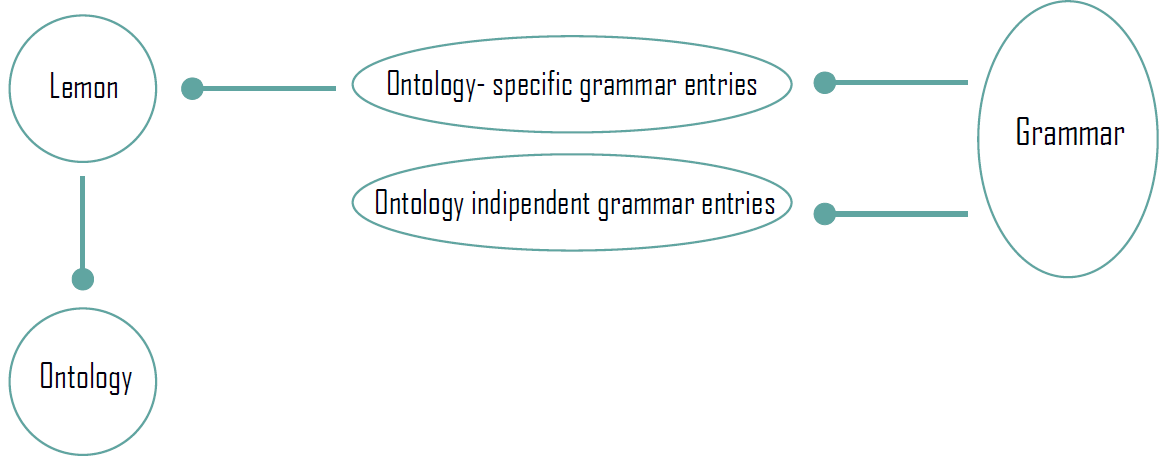
\includegraphics[scale=0.5]{./fig/grammar}
    \label{fig:grammar}
    \caption{The Grammar.}
\end{figure}

Both parts of the grammar use the main linguistic representations or each grammar is represented as a pair of syntactic and semantic representations. As a syntactic representation, Lexicalized Tree Adjoining Grammar (LTAG) is used. As semantic representations we take Dudes.

The first step in generating a grammar from a given ontology is to enrich the ontology with information about its verbalization. To achieve this we leaverage LexInfo, which uses a general frame to create a declarative specification of the lexicon-ontology interface by connecting concepts of the ontology to information about their linguistic realization, i.e. word forms, morphology, sub-categoriziation frames and how syntactic and semantic arguments correspond to each other. The lexical entries specified by LexInfo are then used to generate grammar entries, i.e. indexed LTAG/DUDES.

\subsection{Ontoqa}
The system provides the user with an intuitive interface to submit questions, expressed in English natural language.

The natural language question is processed by the parser to generate the corresponding LTAG/DUDES representation, from which a formal SPARQL query can be obtained.
%After the disambiguation and obtaining of the SLTAG of our universe of speech, we generate a formal query. The formal query will be submitted to the ontology that will return us an answer. 
Finally, the query is submitted to the ontology, thus retrieving the output answer.
The procedure is shown in the Figure.

%The system allows a user to submit, via an intuitive interface, a natural-language question in English.

%Given the question in Natural Language, a parsing is applied that constructs an LTAG derivative tree considering only the syntactic part of the grammatical voices involved.

%Subsequently, syntactic and semantic composition rules apply to the construction of a tree in accordance with the LTAG derivation tree and DUDES semantics.

%In general, what happens is that LTAG provides substitution and adjunction rules while DUDES semantics provides rules as saturation operations that are interpreted as substitutions and a union operation that interprets the adjoin.



\begin{figure}[H]
   \centering
    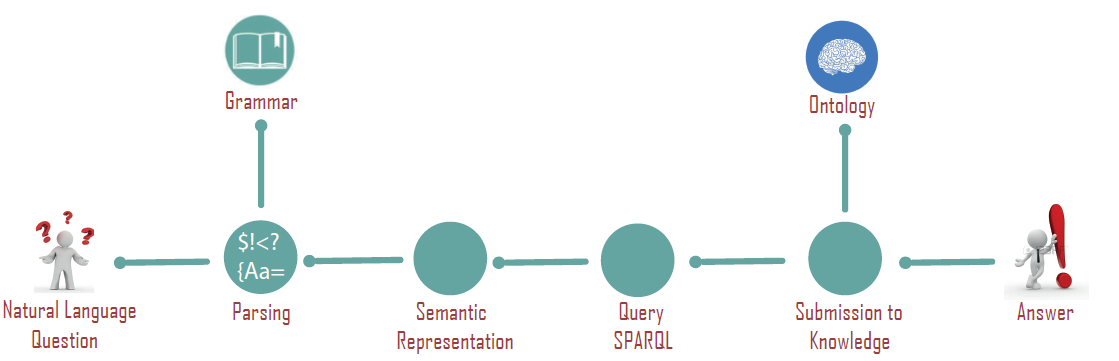
\includegraphics[scale=0.5]{./fig/ontoqa}
    \label{fig:ontoqa}
    \caption{The workflow.}
\end{figure}
\section{Implementation}
\label{sec:implementation}
% ALL

Ontoqa has been realized as a Java\footnote{Oracle Java SE 8} web and standalone application, packaged with Maven.
%
Ontoqa can be executed both as a standalone application and as a web application.
%
All functionalities has been tested carefully against 224 total unit tests.

Ontoqa leverages some well known technologies. Here we present them, giving an idea about how they have been used in our implementation. The reader may refer to the open source code of the project and the corresponding Javadocs to get into the implementation details.


\begin{itemize}
	\item[Ontology] INSERT HERE
	
	\item[Lexicon] The lexical information about ontology is reported in Java by using the APIs provided by the "Semantic Computing Group @ Bielefeld University". The APIs allow the representation of the lemon model in java and the use of lexinfo for generating grammar. The library was manipulated to shape the following lemon properties: 
	\begin{itemize}
		\item Recognition of entries of composite words
		\item Tense and number of different forms of entry 
	\end{itemize}	
Finally, where necessary, a parsing of meaningful terms extracted from paths has been implemented.
The library provided has been to retrieve the ontology represented by the Lemon model from the RDF file and to get a list of Lexical Entry consisting of the most relevant properties shown in the figure:
\begin{figure}[tp]
   \centering
    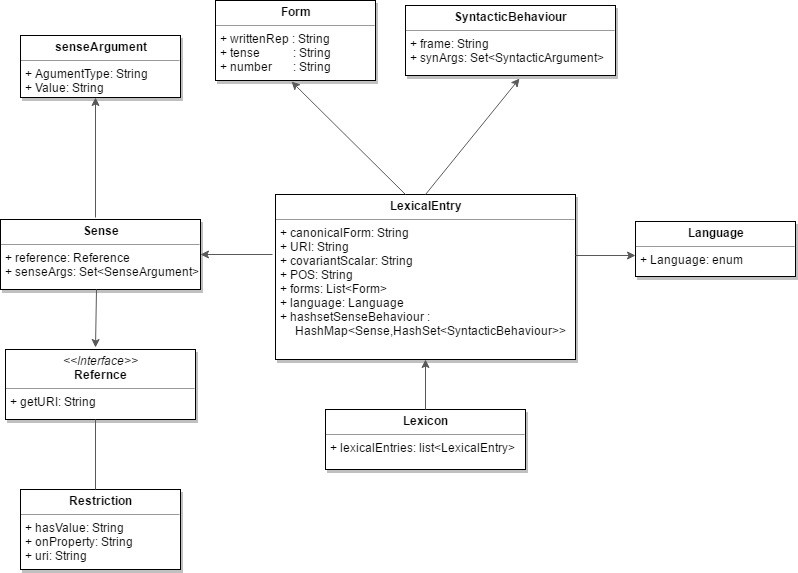
\includegraphics[scale=100]{./fig/lemon}
    \label{fig: lemon}
\end{figure}

	\item[I/O] we used the Jackson core library and data-binding modules to implement data representation in JSON and YAML format.
	
	\item[CLI] we used Apache CLI to implement options and argument parsing for the command line interface.
	
	\item[Web UI] we used AngularJS, JQuery and JavaScript for navigation logic and HTML5 and Bootstrap for the page style.
	
	\item[Web Service] we used Spring Framework and Spring MVC to implement the REST service interface.
	
	\item[Logging] we used SLF4J to implement logging ayer as facade, and Logback as the underlying logging framework.
	
	\item[Development] we used Lombok to implement bean constructors, getter/setters, thus minimizing code redundancy.
	
	\item[Testing] we used JUnit4 to implement unit testing suites.
\end{itemize}


\section{Evaluation}
\label{sec:evaluation}

\lipsum[1]
\section{Further Improvements}
\label{sec:improvements}

A possible improvement could be to extend the library provided by the "Semantic Computing Group @ Bielefeld University" as it does not completely cover the properties of Lemon and Lexinfo, but only the most common properties. 

The second improvement concerns ontology, in particular the redefinition of class hierarchy and the extension of domain knowledge.
\section{Conclusions}
\label{sec:conclusions}

In this work we described Ontoqa, a Q\&A web and standalone application which aims to adapt easily to distinct ontologies and lexicons.
%
The proposed solution leverages ontology-driven NLP through the use of the LTAG/DUDES model and a greedy parsing algorithm aiming to reduce both the syntactic and semantic search space.
%
%
% RESULTS
The experimental results show that our system can answer the benchmark questions, with good performance with respect to both response-time.
%
%
% CONCLUSIONS
Our work shows that ontology alignment through the LTAG/DUDES model permits 
high modularization and generalization of the NLP process.
%
Furthermore, such a model suits well to the design of parsing algorithms that can effectively minimize both the syntactic and semantic search space.


%*******************************************************************************
% Bibliography
%*******************************************************************************
\bibliographystyle{acmreferences}
\bibliography{ref/biblio}

\end{document}
